%\documentclass[tikz,border=5mm,convert={outfile=\jobname.png}]{standalone}
\documentclass{standalone}
\usepackage{tikz}
\usetikzlibrary{calc}
\begin{document}
	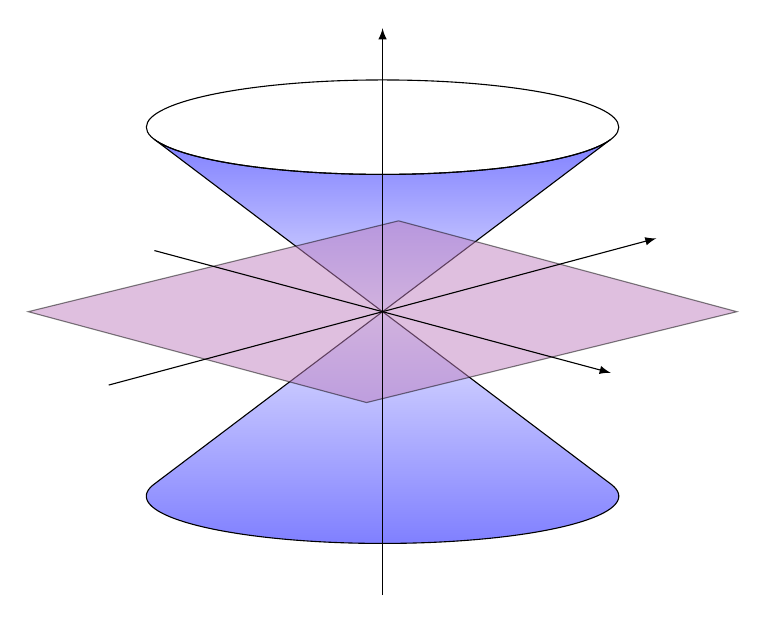
\begin{tikzpicture}
		\def\a{3}
		\def\xo{2.9}
		\pgfmathsetmacro{\b}{\a/5}
		\def\f(#1){\b *sqrt((\a)^2-(#1)^2)/\a}%Công thức hàm số
		\def\fdh(#1){-\b *(#1)/(\a *sqrt( (\a)^2 -(#1)^2))}%Công thức đạo hàm
		\pgfmathsetmacro{\yo}{\f(\xo)}
		\pgfmathsetmacro{\fdho}{\fdh(\xo)}
		\pgfmathsetmacro{\go}{acos(\xo/\a)}
		\pgfmathsetmacro{\h}{\yo-\fdho *\xo}
		\draw[bottom color=blue!50,top color=blue!10,shift={(0,-\h)}] plot[domain=\go:-180-\go,smooth,samples=200,variable=\t]({\a *cos(\t)},{\b *sin(\t)})--(0,\h)--cycle;
		\draw[bottom color=blue!10,top color=blue!50,yscale=-1, shift={(0,-\h)}] plot[domain=\go:180-\go,smooth,samples=200,variable=\t](({\a *cos(\t)},{\b *sin(\t)})--(0,\h)--cycle;
		\draw[yscale=-1,shift={(0,-\h)}] (0:0) ellipse ({\a} and {\b});
		\draw[fill=violet!50, opacity=0.5] (-180:1.5*\a)--(-100:\h/2)--(0:1.5*\a)--(80:\h/2)--cycle;
		\draw [-latex] (270:\a+\b)--(90:\a+\b);
		\draw [-latex] (195:\a+\b)--(15:\a+\b);
		\draw [-latex] (165:\a)--(-15:\a);
	\end{tikzpicture}
\end{document}